\documentclass[9pt, preprint]{sigplanconf} % <<<

% Keep fontenc and inputenc them in this order.
\usepackage[T1]{fontenc}
\usepackage[latin1]{inputenc}

\usepackage{amsmath}
\usepackage{amssymb}
\usepackage{booktabs}
\usepackage{graphics}
\usepackage{microtype}  % do not remove
\usepackage{multirow}
\usepackage{proof}
\usepackage{pygmentize}
\usepackage{rgalg}
\usepackage{tikz}
\usepackage{xcolor}
\usepackage{xspace}

\usepackage{tikz}
\usetikzlibrary{arrows,positioning,fit,backgrounds,shadows,calc}

\usepackage[colorlinks]{hyperref} % keep it last to avoid some warnings

\RecustomVerbatimEnvironment{Verbatim}{BVerbatim}{}
\definecolor{darkred}{rgb}{0.4,0,0}
\definecolor{darkblue}{rgb}{0,0,0.4}
\definecolor{verylightgray}{rgb}{0.9,0.9,0.9}
\definecolor{lightblue}{rgb}{0,0,0.9}
% comment the next line for printing
\hypersetup{colorlinks,linkcolor=darkblue,citecolor=darkblue,urlcolor=darkblue}
\hypersetup{
  pdftitle={Runtime Checking with Register Automata},
  pdfauthor={Radu Grigore and Dino Distefano and Rasmus Lechedahl Petersen}}

\title{Runtime Checking with Register Automata}
%\authorinfo{Authors info whitheld for double-blind submission}
\authorinfo{Radu Grigore}
           {Queen Mary University of London}
           {rgrig@eecs.qmul.ac.uk}
\authorinfo{Dino Distefano}
           {Queen Mary University of London}
           {ddino@eecs.qmul.ac.uk}

\authorinfo{Rasmus Lerchedahl Petersen}
           {Microsoft Research}
           {rusmus@eecs.qmul.ac.uk}

\renewcommand{\sectionautorefname}{Section}
\renewcommand{\subsectionautorefname}{\sectionautorefname}

\newcommand{\noterg}[2]{\textcolor{gray}{[\textcolor{red}{#1}: #2]}}
\newcommand{\rg}[1]{\noterg{rg}{#1}}
\newcommand{\rlp}[1]{\noterg{rlp}{#1}}
\newcommand{\dd}[1]{\noterg{dd}{#1}}
\newcommand{\dinocomment}[1]{\dd{#1}}

\newcommand{\B}{\ensuremath{\mathbb{B}}}
\newcommand{\N}{\ensuremath{\mathbb{N}}}
\newcommand{\delimitVerbatim}{\par\nobreak\smallskip\noindent}
\newcommand{\error}{\ensuremath{\textcolor{darkred}{\mathtt{error}}}\xspace}
\newcommand{\eval}[1]{[[#1]]}
\newcommand{\pattern}[1]{\ensuremath{\mathtt{\underline{#1}}}}
\newcommand{\pmap}{\rightharpoonup}
\newcommand{\set}[1]{\ensuremath{\mathsf{#1}}}
\newcommand{\start}{\ensuremath{\mathtt{start}}\xspace}
\newcommand{\verbline}[2][]{\[\text{\Verb@#2@}#1\]}

\newcommand{\eqquote}[2]{{%
  \refstepcounter{equation}\label{#2}%
  \setbox0=\vbox{\advance\hsize by-3\parindent\noindent\em#1}%
  \newdimen\x\x=\ht0 \advance\x by\dp0%
  \setbox1=\vbox to\x{\vss\hbox{(\arabic{equation})}\vss}%
  \leavevmode\\[1ex]%
  \hbox to\hsize{\hskip 1.5\parindent\box0\hfil\box1}%
  \\[1ex]}}

% rg: I tend to give grammars in BFS order
\def\grammar#1{{
  \footnotesize
  \def\b##1{{\rm\Verb@##1@}}\def\*{$^*$}\def\?{$^?$}\def\({$($}\def\){$)$}
  \def\|{$\mid$}\def\+{$^+$}
  \smallskip
  \hbox to\hsize{\hfil\vbox{\halign{\hfil\it##&$\;::=\;$\it##\hfil&\qquad\rm##\hfil\cr#1}}\hfil}
  \smallskip
}}


\newtheorem{definition}{Definition}
\newtheorem{example}{Example}
\newtheorem{notation}{Notation}

% For the final version, switch then comment-status of the following lines.
%\overfullrule=5pt
\renewcommand{\noterg}[2]{}

\showboxdepth=10
\showboxbreadth=30
% >>>
\begin{document}
\maketitle
\begin{abstract} % <<<
We introduce a new technique for checking temporal safety properties of Java programs.
Our approach is based on a new specification language for an extended class of {\em register automata} able to express complex properties of systems involving multiple interacting objects.
The specifications are then used to instrument Java bytecode so that their violations can be automatically detected at runtime.
We have validated our technique by checking several safety properties on large open source projects.
\end{abstract}

% >>>
\section{Introduction} % <<<
Interaction of objects is at the core of the object-oriented paradigm.
Programmers often have an informal and global understanding of how objects relate.
Consider for example Java collections.
A typical property one would want to state~is:
\eqquote{If one iterator modifies its collection, then other existing iterators of the same collection become invalid, which means they cannot be used further.}{q:concur-it}
The formalization of the above constraint is non-trivial since it needs to keep track of {\em several objects} (at least two iterators, and one collection) and their {\em interaction over time}.

In this paper we define TOPL (Temporal Object-oriented Property Language), a language for specifying temporal safety properties of Java programs.
Similar formalisms used for runtime checking of Java programs include typestates~\cite{dblp:journals/scp/harel87} and tracematches~\cite{dblp:conf/oopsla/allanachklmsst05}.
Unlike those, TOPL is based on an automata formalism designed for {\em infinite alphabets}~\cite{dblp:conf/csl/segoufin06}.
In the context of program analysis the alphabet is the set of program values.
This set is infinite since there is no bound on the number of instantiations.
There are several such automata formalisms;
TOPL is an extension of register automata~\cite{dblp:journals/tcs/kaminskif94}.
%For standard finite-state automata, nondeterminism does not increase expressivity;
%with infinite alphabets, nondeterminism does increase expressivity.
For standard finite-state automata, nondeterminism does not increase expressivity;
however combining  infinite alphabets and nondeterminism gives strictly more expressive automata. 
Runtime checkers based on typestates~\cite{arnold:2008}, tracematches, or LTL~\cite{dblp:conf/oopsla/chenr07} are essentially deterministic, for speed.
We chose to give TOPL nondeterministic semantics.

We also introduce a technique for automatic runtime checking of TOPL properties.
This technique provides to programmers a flexible methodology to enforce the safety properties with which the code should comply.
Currently, the only option for the developer is to insert explicit checks directly in the code.
For example, every iterator and every collection in \texttt{java.util} contains checks concerning the example property~\eqref{q:concur-it}.
It is impossible to turn off these checks, even if one has a proof that a certain program correctly uses the library.
Because these checks are always active, their overhead must be very low.
As a result, when a check fails, the user is not provided with an error trace.
Also, such checks are difficult to write and to maintain.
Other libraries document such temporal constraints only in (informal) comments.
With TOPL, the programmer (formally) describes the properties in one place, which is separate from the code. 
This description serves as a rigorous documentation of which safety properties are enforced on the program.
Then it is the job of the TOPL compiler to insert the appropriate checks into the Java bytecode of the program.
The execution is monitored and violations are reported as traces of events.
The programmer has the ability to tune the overhead by choosing how many objects to track, for how long to remember past events, and a few other parameters.
For example, during testing they could allow for a very high overhead, whereas they could choose to deploy the bytecode without any inserted check.

\paragraph{Contributions.}
In summary, the contributions of this paper are:
\begin{itemize}
\item We define the TOPL specification language, which is tailored to express properties involving object interactions over time in a way that is familiar to Java programmers.
\item We give precise formal semantics for TOPL, making it suitable for program analysis, both static and dynamic.
\item We define a precise relation between TOPL's semantic model and register automata. 
\item We introduce a technique to automatically check at runtime violations of TOPL properties in Java programs.

\item We discuss the implementation of our technique.
\item We report the results of using our tool on large open-source projects. The results are encouraging: we have found
violations of properties, and we have observed an acceptable runtime overhead. 
\end{itemize}

The paper is organized as follows.
\autoref{sec:results} gives the experimental results.
\autoref{sec:examples} introduces the TOPL language with examples.
\autoref{sec:semantics} gives TOPL's semantics.
\autoref{sec:ra-topl} describes the relationship between TOPL automata and register automata.
\autoref{sec:implementation} describes a the interesting aspects of the implementation.
\autoref{sec:related} discusses related work.
Finally, \autoref{sec:conclusions} concludes the paper and describes our plans for future work.

% >>>
\section{Experimental Results}\label{sec:results} % <<<

Our interest in temporal properties of object-oriented programs was initially purely theoretical.
But we implemented our technique to ensure we are not dismissing an important issue as merely engineering.
In particular, without an implementation it is hard to judge if the performance penalty is acceptable.

\subsection{Methodology} % <<<

We expect our technique to be most useful during development.
Library writers will document temporal constraints in TOPL, not just in English.
Each library will have a testing version, obtained by instrumenting the bytecode with the TOPL properties.
Users will use the testing version of the library to ensure they use it correctly.
By the time end-users see the application, most temporal bugs are gone.
Back in the real world, we too would like to know if such a scenario is likely.
Alas, observing the effect of using TOPL during the life-time of a real project is rather time consuming.
We have to settle for less.

We measure the overhead on the test suite DaCapo~\cite{dblp:conf/oopsla/dacapo}, version~9.12.
DaCapo is a collection of automated tests that exercise large portions of code from open-source projects.
We focus on $3$~projects that are still widely developed and used: Tomcat, H2, and PMD\null.
These are all mature projects with many users.
DaCapo itself was used for many experiments by the research community.
Hence, we do not expect to find any bugs, but aim to measure the overhead.
For each project we write a few TOPL properties that encode information that exists in the code comments.
In fact, we identify these properties by searching the code for words with temporal connotations, such as `before' and `after'.

We measure both the time overhead and the space overhead.
The time overhead is reported measured for various configurations of the checker, and also for the original bytecode, with no instrumentation whatsoever.

All experiments are performed on the same machine.
The operating system kernel is Linux~2.6.32.
The Java VM has version~1.6.0\_20.
The processor is Intel i5 with $4$~cores at $3.33\rm\,GHz$.
The total system memory is $4\rm\,GiB$.

% >>>
\subsection{A Bug's Death} % <<<

The interface \texttt{ServletResponse} from Tomcat contains methods \texttt{getWriter} and \texttt{getOutputStream}.
The documentation of \texttt{getWriter} states that ``either this method or \texttt{getOutputStream} may be called to write the body, not both''.
We initially interpreted this comment as follows.
\eqquote{It is illegal to call both the method {\tt getWriter} and the method {\tt getOutputStream} on the same instance of {\tt ServletResponse}.}{eq:prop-ws-strong}
The TOPL checker reported many violations of~\eqref{eq:prop-ws-strong}.
We were not too surprised because we were unsure of the intended meaning of the comment.
We were surprised, however, that sometimes a {\tt null} dereference occurred in DaCapo itself.
We investigated.
The statement that threw a {\tt null}-pointer exception was the following:
\begin{align}\label{eq:npe-src}
\text{\Verb@if (log != null) log.write(b);@}
\end{align}
It must be that a concurrent thread sets {\tt log} to~{\tt null}.
The statement is located in the method {\tt write} of the class {\tt TeeOutputStream}.
The only method that sets {\tt log} to~{\tt null} is {\tt closeLog}, from the same class.
So, we wrote a TOPL property saying that \textit{executions of {\tt write} and {\tt closeLog} must not overlap in time}, and we asked for error reports that include call stacks.
Indeed, DaCapo's main loop sometimes calls {\tt closeLog} while the Tomcat server is printing.
%XXX\rg{Put here a trace for the error.}

TOPL helped us find a concurrency bug in the infrastructure of DaCapo.
First, the bytecode instrumented by TOPL helped us notice the problem.
The reason is \emph{not} that a certain interleaving became more likely.
Bug~2934521 of DaCapo mentions that exceptions of the Tomcat benchmark are silently ignored.
This is why the {\tt null}-dereference was not noticed before.
The TOPL checker tried to report an unrelated issue to {\tt System.err}.
DaCapo had redirected the standard error stream to its own class, which faulted.
TOPL caught the error and reported it as an internal issue, because no exceptions should be thrown while running the TOPL checker.
This is why we noticed the {\tt null}-dereference.
Second, TOPL helped us identify the data race.
It was easy to notice that statement~\eqref{eq:npe-src} should be atomic.
However, it would have been more difficult to figure out which threads exactly used the stream simultaneously.

We then tried a weaker version of property~\eqref{eq:prop-ws-strong}:
\eqquote{The stream and the writer of a response cannot both be used.}
{eq:prop-ws-weak}
This property involves three related objects.
The full TOPL property appears in~\autoref{fig:tomcat-prop}.
It turns out this property is also violated.
After reading the code to which the error traces pointed at, we noticed that the comments of some implementing classes weaken the contract:
They say that the stream and the response cannot be used without an intervening {\tt reset}.
In this case the comments on the interface {\tt ServletResponse} are arguably wrong, rather than the code.
This brings out another advantage of TOPL:
Since TOPL properties are processed by tools, they are less likely to become out-of-sync with the code.

% >>>
\subsection{Benchmarks} % <<<

All three benchmarks are large open-source projects with many users and active developers.
The versions were current in 2009 when DaCapo-9.12 was released.

\paragraph{Tomcat 6.0.20.}
Tomcat is a servlet server; so, highly concurrent.
Servlets are Java programs that run in a webserver, extract data from {\tt ServletRequest}s , and send data into {\tt ServletResponse}s.
A response has two associated incoming channels: a stream and a writer.
The stream and the writer should not both be used.
Property~\eqref{eq:prop-ws-strong} is a strong interpretation of this constraint;
property~\eqref{eq:prop-ws-weak} is a weak interpretation of this constraint.
A response could be forwarded once the servlet sent data to it.
But, the servlet must commit a response before forwarding it, by calling {\tt fulsh} on the stream, on ther writer, or on the response itself.
This is the other property we checked.

\paragraph{H2 1.2.121.}
H2 is a database server.
We checked four properties for it.
Three properties express constraints on the order in which the methods of an interface may be called.
For example, a client should not attempt to ask for a row from a cursor that did not advance;
that is, for the interface {\tt Cursor}, the method {\tt next} must be called before calling method {\tt getSearchRow}.
The fourth property describes the contract of the class {\tt SysConstants}.
This class reads environment variables when it is loaded.
Its comments say that it is legal for a program to set these environment variables using the method {\tt System.setProperty}, provided that this is done before the Java VM loads the class {\tt SysConstants}.
It is easy to specify this property because TOPL intentionally treats the special methods {\tt <init>} and {\tt <clinit>} as if they are normal methods.

\paragraph{PMD 4.2.5.}
PMD looks for bugs, dead code, and a few other problems in Java code.
We checked five properties for it.
One of the five involves two objects:
A scope should be asked what is the definition of a name only if it already replied that it knows the name.

% >>>
\subsection{Overhead} % <<<

Instrumenting DaCapo, which has $160\rm\,MiB$, takes $7$~minutes.
One needs to instrument once for a given set of properties, because instrumentation is property-directed.
A change of a runtime parameter, such as the maximum number of tracked active states, requires recompiling the TOPL checker, but does not require re-instrumenting.

\paragraph{Space.}
Estimates of heap size showed no significant increase in memory use.
We used a simple method.
The heap of a Java program has three parts: used, garbage, and free.
The class {\tt Runtime} from the package {\tt java.lang} provides an estimate of the total size and of the free size.
The difference is an estimate of the used size, provided the garbage was collected immediately before.
We put this code, which estimates memory use, in the TOPL checker.
So, strictly speaking we did not estimate the memory use without the checker.
However, we used as a baseline a run that tracked no active state.
We also run the estimate for various other counts of tracked active states.

\paragraph{Time.}
\autoref{table:overhead} summarizes the experimental results.
The reference column shows the running time without any instrumentation.
A timeout signifies a time greater than the reference time~$\times100$.
All reported times are averaged over $10$~runs, and are accompanied by the unbiased estimate of standard deviation.
The TOPL checker essentially simulates a nondeterministic register automaton.
In theory the set of active states is unbounded, but we impose a size limit on it.
The table reports the running times for the instrumented bytecode when the size limit is $0$, $10^1$, $10^2$, $10^3$, and~$10^4$.

For tomcat the running time is essentially the same when tracking $\le10^4$ active states as it is when tracking $\le10^3$ active states.
This indicates that $\le10^3$ active states already exhaustively check the given properties.
For h2 the running time is more than $\times1.4$ the reference time even when the TOPL checker is not tracking any active state.
This indicates that we instrumented a simple method that runs often.

\begin{table*}[t]\centering
\begin{tabular}{@{}rr@{}lr@{}lr@{}lr@{}lr@{}lr@{}l}
  &&
  & \multicolumn{10}{c}{Number of tracked active states} \\ \cmidrule{4-13}
& \multicolumn{2}{c}{reference}
  &\multicolumn{2}{c}{$\le0$}
  &\multicolumn{2}{c}{$\le10^1$}
  &\multicolumn{2}{c}{$\le10^2$}
  &\multicolumn{2}{c}{$\le10^3$}
  &\multicolumn{2}{c}{$\le10^4$} \\ \midrule
tomcat
  & $5.3$ & $\pm0.1$
  & $5.4$ & $\pm0.1$
  & $5.6$ & $\pm0.2$
  & $9.0$ & $\pm0.3$
  & $43.5$ & $\pm1.2$
  & $43.9$ & $\pm1.0$ \\
pmd
  & $5.2$ & $\pm0.4$
  & $5.4$ & $\pm0.2$
  & $12.2$ & $\pm0.3$
  & $47.7$ & $\pm10.7$
  & \multicolumn{2}{c}{timeout}
  & \multicolumn{2}{c}{timeout}
  \\
h2
  & $6.6$ & $\pm0.2$
  & $9.5$ & $\pm0.2$
  & $130.1$ & $\pm12.2$
  & \multicolumn{2}{c}{timeout}
  & \multicolumn{2}{c}{timeout}
  & \multicolumn{2}{c}{timeout}
  \\
\end{tabular}
\caption{
  Experimental Results.
  Times are in seconds, averaged over $10$~runs.
}\label{table:overhead}
\end{table*}

% >>>
% >>>
\section{TOPL by Example} \label{sec:examples} % <<<

In this section, which is based on our previous article~\cite{our-fool2011},  we introduce TOPL in an informal way by means of examples.


\subsection{Iterators Step by Step} \label{sec:examples.steps} % <<<

Consider the program in \autoref{fig:first.java}. The last statement violates the property of the introduction, therefore throwing an exception.
There are two iterators on the same collection, one of them modifies the collection, and this invalidates the other iterator.
Such properties are often explained using diagrams that are sometimes precise, but not expressive enough~\cite{dblp:journals/scp/FieldGRY05,dblp:conf/issta/FinkYDRG06} or sometimes expressive, but imprecise~\cite{dblp:conf/oopsla/bierhoffa07,dblp:conf/oopsla/naeeml08,dblp:conf/sigsoft/boddenlh08,dblp:conf/ecoop/bierhoffba09}.
\autoref{fig:first.topl} (top)  captures precisely a temporal property involving three interacting objects.
Below the same property is described in the textual form of TOPL, isomorphic to the diagram.
The first line is an observe directive that declares that we are
interested in all method calls (denoted by the wild card *) on
instances of \Verb@java.util.Collection@ and \Verb@java.util.Iterator@ \emph{and} all those that override them.

In a TOPL property, vertices have identifiers (\texttt{start}, \texttt{one}, \texttt{two}, \dots);
transitions have labels ($\pattern I:=\pattern C.\mathtt{iterator}()$, \dots).
There are two special vertices: \start, from where the execution begins; and \error, where the execution ends.
Labels resemble the shape of statements that enable the corresponding transition.

We understand a TOPL property as an automaton that monitors the
program, by making transitions when the program executes corresponding
statements. If the program drives the automaton to the error state in
this manner, then the program violates the property.

\begin{figure}[t] % first example <<<
\begin{Verbatim}[commandchars=\\\{\}]
\PY{k+kn}{import} \PY{n+nn}{java.util.*}\PY{o}{;}
\PY{k+kd}{public} \PY{k+kd}{class} \PY{n+nc}{IncorrectIteratorUse} \PY{o}{\PYZob{}}
  \PY{k+kd}{public} \PY{k+kd}{static} \PY{k+kt}{void} \PY{n+nf}{main}\PY{o}{(}\PY{n}{String}\PY{o}{[}\PY{o}{]} \PY{n}{args}\PY{o}{)} \PY{o}{\PYZob{}}
    \PY{n}{List}\PY{o}{<}\PY{n}{Integer}\PY{o}{>} \PY{n}{c} \PY{o}{=} \PY{k}{new} \PY{n}{ArrayList}\PY{o}{<}\PY{n}{Integer}\PY{o}{>}\PY{o}{(}\PY{o}{)}\PY{o}{;}
    \PY{n}{c}\PY{o}{.}\PY{n+na}{add}\PY{o}{(}\PY{l+m+mi}{1}\PY{o}{)}\PY{o}{;} \PY{n}{c}\PY{o}{.}\PY{n+na}{add}\PY{o}{(}\PY{l+m+mi}{2}\PY{o}{)}\PY{o}{;}
    \PY{n}{Iterator}\PY{o}{<}\PY{n}{Integer}\PY{o}{>} \PY{n}{i} \PY{o}{=} \PY{n}{c}\PY{o}{.}\PY{n+na}{iterator}\PY{o}{(}\PY{o}{)}\PY{o}{;}
    \PY{n}{Iterator}\PY{o}{<}\PY{n}{Integer}\PY{o}{>} \PY{n}{j} \PY{o}{=} \PY{n}{c}\PY{o}{.}\PY{n+na}{iterator}\PY{o}{(}\PY{o}{)}\PY{o}{;}
    \PY{n}{i}\PY{o}{.}\PY{n+na}{next}\PY{o}{(}\PY{o}{)}\PY{o}{;} \PY{n}{i}\PY{o}{.}\PY{n+na}{remove}\PY{o}{(}\PY{o}{)}\PY{o}{;} \PY{n}{j}\PY{o}{.}\PY{n+na}{next}\PY{o}{(}\PY{o}{)}\PY{o}{;}
  \PY{o}{\PYZcb{}}
\PY{o}{\PYZcb{}}
\end{Verbatim}

\caption{A first example: Java code}
\label{fig:first.java}
\end{figure}
%
\begin{figure}[t]
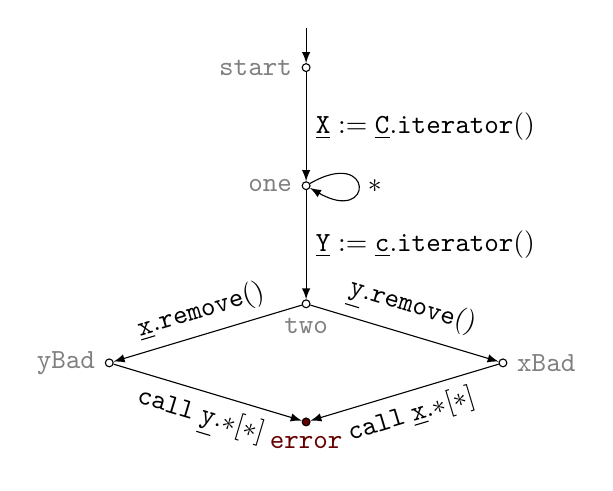
\begin{tikzpicture}
  \def\x{2.5}
  \def\y{1.5}
  \tikzset{vertex/.style={draw,circle,inner sep=1pt}}
  \tikzset{transition/.style={->,>=latex}}
  \tikzset{every label/.style={gray}}
  \node[vertex] (start) at (0,0) [label=left:\texttt{start}] {};
  \node[vertex] (one) at (0,-1*\y) [label=left:\texttt{one}] {};
  \node[vertex] (two) at (0,-2*\y) [label=below:\texttt{two}] {};
  \node[vertex] (xBad) at (1*\x,-2.5*\y) [label=right:\texttt{xBad}] {};
  \node[vertex] (yBad) at (-1*\x,-2.5*\y) [label=left:\texttt{yBad}] {};
  \node[vertex,fill=darkred] (error) at (0,-3*\y) [label=below:\textcolor{darkred}{\texttt{error}}] {};
  \draw[transition] (0,0.5)--(start);
  \draw[transition] (start)--node[right]{$\pattern X:=\pattern C.\mathtt{iterator}()$} (one);
  \draw[transition] (one) .. controls +(30:1cm) and +(-30:1cm) .. node[right]{$*$} (one);
  \draw[transition] (one)--node[right]{$\pattern Y:=\pattern c.\mathtt{iterator}()$} (two);
  \draw[transition] (two) -- node[sloped,above]{$\pattern y.\mathtt{remove}()$} (xBad);
  \draw[transition] (two)--node[sloped,above]{$\pattern x.\mathtt{remove}()$} (yBad);
  \draw[transition] (xBad)--node[sloped,below]{$\mathtt{call}\;\pattern x.{*}[*]$} (error);
  \draw[transition] (yBad)--node[sloped,below]{$\mathtt{call}\;\pattern y.{*}[*]$} (error);
\end{tikzpicture}
\\[2ex]
\begin{Verbatim}[commandchars=\\\{\}]
property InvalidateOtherIterators
  observe <java.util.\{Collection,Iterator\}.*>
  prefix <java.util.\{Collection,Iterator\}>
  start -> start: *
  start -> one:  \pattern{X} := \pattern{C}.iterator()
  one -> one:    *
  one -> two:    \pattern{Y} := \pattern{c}.iterator()
  two -> yBad:   \pattern{x}.remove()
  two -> xBad:   \pattern{y}.remove()
  yBad -> error: call \pattern{y}.*[*]
  xBad -> error: call \pattern{x}.*[*]
\end{Verbatim}
\caption{Property {\tt InvalidateOtherIterators} in diagram (above) and textual form (below).
}
\label{fig:first.topl}
\end{figure}
%
\begin{figure}[t]
{\def\s#1{\text{\Verb@#1@}}
 \def\m#1{\PY{n+na}{#1}}
 \def\t#1{\mathtt{#1}}
 \def\cmt#1{\textcolor{gray}{\text{// #1}}}
\begin{align*}
&\{\;(\start,[])\;\} \\
&\s{Iterator<Integer> i = c.\m{iterator}();}  \quad \cmt{\bf \it Step 1} \\
&\cmt{Assume {\tt c} holds $1$, and {\tt i} holds $2$ } \\
& \begin{aligned}
  \{\;&(\start,[]),\
      &(\t{one},[c:1,x:2])\;\}
  \end{aligned}\\
&\s{Iterator<Integer> j = c.\m{iterator}();}  \quad \cmt{\bf \it Step 2} \\
&\cmt{Assume {\tt j} holds $3$} \\
& \begin{aligned}
  \{\;&(\start,[]),\
      &(\t{one},[c:1,x:2]),\
      &(\t{one},[c:1,x:3]),\
   \end{aligned}\\
& \begin{aligned}   
      & \quad (\t{two},[c:1,x:2,y:3])\;\}
  \end{aligned}\\
&\s{i.\m{next}();} \quad \cmt{\bf \it Step 3} \\
& \begin{aligned}
  \{\;&(\start,[]),\
      &(\t{one},[c:1,x:2]),\
      &(\t{one},[c:1,x:3]),\
   \end{aligned}\\
& \begin{aligned}   
      & \quad (\t{two},[c:1,x:2,y:3])\;\}
  \end{aligned}\\
&\s{i.\m{remove}();} \quad \cmt{\bf \it Step 4}  \\
& \begin{aligned}
  \{\;&(\start,[]),\
      &(\t{one},[c:1,x:2]),\
      &(\t{one},[c:1,x:3]),\
   \end{aligned}\\
& \begin{aligned}   
      & \quad (\t{yBad},[c:1,x:2,y:3])\;\}
  \end{aligned}\\
&\s{j.\m{next}()} \quad \cmt{\bf \it Step 5}  \\
& \begin{aligned}
  \{\;&(\start,[]),\
      &(\t{one},[c:1,x:2]),\
      &(\t{one},[c:1,x:3]),\
   \end{aligned}\\
& \begin{aligned}   
      & \quad (\error,[c:1,x:2,y:3])\;\}
  \end{aligned}\\
\end{align*}}
\caption{Running trace of {\tt InvalidateOtherIterators}. Lines \{in curly brackets\} describe automaton's states;
lines in \texttt{monotype} show executing statements;
// are comments.}
\label{fig:first.steps}
\end{figure} % >>>
\autoref{fig:first.steps} shows an execution of the program in \autoref{fig:first.java} and an automaton for \texttt{InvalidateOtherIterators}.
At a given moment, the automaton has a set of active states.
A state is a pair of a vertex and a store.
The store is a memory that holds (automaton) variables.
Technically, it is a finite partial map from variables to values.
We write $[k_1:v_1,k_2:v_2]$ for the finite partial map that maps key~$k_1$ to value~$v_1$, and key~$k_2$ to value~$v_2$.
The empty map is denoted by~$[]$.

The automaton has variables $x$,~$y$, and~$c$.
At vertex \texttt{one} the variables $x$~and~$c$ are initialized;
at \texttt{two} the variables $x$,~$y$, and~$c$ are initialized.
At vertex \texttt{one} $x$~is an iterator for a collection~$c$, and
at \texttt{two}, $x$~and~$y$ are both two iterators for the same collection~$c$.
Notice that~\Verb@c@ is a program variable whereas~$c$ is an automaton variable.
The same name was chosen because the two variables always hold the same value in this example.
In general, however, program variables and automaton variables live in different name-spaces, and may hold different values.

To avoid confusion, program variables are typeset in \Verb@monotype@ (\Verb@c@,~\Verb@i@,~\Verb@j@).
Automaton variables are typeset in \textit{italics} ($c$,~$x$,~$y$) and do \emph{not} appear in the property.
Instead, automaton variable \emph{patterns} appear in the property, and they are typeset in \texttt{\underline{underlined monotype}} (\pattern c,~\pattern C, \pattern x, \pattern X, \pattern y,~\pattern Y).
The interaction between patterns and the automaton's memory is as follows: uppercase patterns write to the automaton memory, and lowercase patterns read from the automaton memory and act as a guard on the transition.

We now illustrate all this by going through the execution step by
step.

\paragraph{Step~1.}

Initially, only the state $(\start,[])$ is active.
The outgoing transition of vertex \start is labeled by $\pattern X:=\pattern{C}.\mathtt{iterator}()$ and the first executed statement is \verbline[.]{i = c.\PY{n+na}{iterator}()}
A method call matches a label when
\begin{itemize}
\item[(a)] the called method matches the method pattern, and
\item[(b)] the program values match their corresponding patterns.
\end{itemize}
By definition, any value matches an Uppercase pattern.
So here, the values of \Verb@i@~and~\Verb@c@ match the patterns \pattern X~and~\pattern C.
The method itself also matches the method pattern.
For simplicity, we ignore argument types and identify Java methods only by their fully qualified name and their arity.
The called method \texttt{iterator} is in the class \texttt{ArrayList} and has arity~$1$.
We identify it as follows.
\verbline{java.lang.ArrayList.iterator[1]}
The \texttt{prefix} directives, allows us to write the method pattern \Verb@iterator[1]@
and have it expanded to the following:
\begin{align*}
&\text{\Verb@java.util.Collection.iterator[1]@} \\
&\text{\Verb@java.util.Iterator.iterator[1]@}
\end{align*}
Similar to the \texttt{observe} directives, it means that these two methods \emph{and} all those that override them match.
Here, \texttt{ArrayList} implements \texttt{Collection} and so\\
\texttt{ArrayList.iterator} matches.

Thus, all conditions are met to enable the transition from \start to \texttt{one}.
When the transition is performed, the values that matched \pattern X~and~\pattern C are written in the automaton variables $x$~and~$c$.
For concreteness, let us assume these values are $1$~and~$2$. When the
program runs, these values will be the memory addresses of the objects
\Verb@c@ and \Verb@i@, so $1$ and $2$ are unlikely values, but for the
example they suffice.
After the transition is performed, the state $(\mathtt{one},[c:1,x:2])$ is active.
The state $(\start,[])$ remains active because the transition \verbline{start -> start: *} is also enabled and performed.

\paragraph{Step~2.}
For the second step, the statement to be executed is \verbline[.]{j = c.\PY{n+na}{iterator}()}
Now we need to consider, in turn, the two active states \[\{(\start,[])\quad\text{and}\quad(\texttt{one},[c:1,x:2])\}\]
For $(\start,[])$ the same reasoning as for step 1 holds, so the states $(\start,[])$ and $(\mathtt{one},[c:1,x:3])$ are active after step~2.
Note that now the automaton variable~$x$ remembers the value of the program variable~{\tt j}.
For $(\texttt{one},[c:1,x:2])$ we look at the outgoing transitions from vertex {\tt one}.
\begin{align*}
\text{\Verb@one -> one@} &: * \quad \mbox{ and } \quad \\
\text{\Verb@one -> two@} &: \text{\Verb@\pattern Y := \pattern c.iterator()@}
\end{align*}
The first transitions is always enabled, and performing it keeps states with vertex \texttt{one} active.
The second transitions has two patterns, \pattern Y~and~\pattern c.
The uppercase pattern~\pattern Y always matches, whereas
pattern \pattern c matches only the value held by the automaton variable~$c$.
In this case, $c$ was set in the previous step to the value of the program variable~\texttt{c}.
Therefore, the transition from~\Verb@one@ to~\Verb@two@ is performed and the state $(\mathtt{two},[c:1,x:2,y:3])$ is activated.

\paragraph{Step~3.}

The third step involves the statement
\[\text{\Verb+\PY{n}{i}\PY{o}{.}\PY{n+na}{next}\PY{o}{(}\PY{o}{)}\PY{o}{;}+}\]
which matches no label of outgoing transitions of the currently active vertices (that is, \start, {\tt one}, and {\tt  two}).
Therefore, although the program proceeds, the set of active states of the automaton remains unchanged.

\paragraph{Step~4.}

In the fourth step, the transition $\texttt{two}\to\texttt{yBad}$ is performed.
Notice that the pattern $\pattern{x}.\mathtt{remove}()$ does not have a left-hand side, which simply means that the returned value is irrelevant for this transition.
The states corresponding to vertices \start and {\tt one} remain unchanged, because their outgoing transitions are disabled.
However,  the outgoing transition of state {\tt two} is enabled, and therefore {\tt yBad} becomes active.

\paragraph{Step~5.}

For the fifth and final step, the statement to be executed is \verbline[.]{j.\PY{n+na}{next}()}
The label of the outgoing transition  \[\mathtt{call}\;\pattern{y}.{*}[*]\] of the active state $(\texttt{yBad},[c:1,x:2,y:3])$
has two distinguishing features: the~$*$ as a method name and the tag \texttt{call}.
As before, in order to match the method name, the prefixes
\Verb@java.util.Collection.*[*]@ as well as \Verb@java.util.Iterator.*[*]@
are prepended.
Then the $*$s are expanded, taking into account the \texttt{CLASSPATH}.
One expansion, \Verb@java.util.Iterator.next@, is indeed
overridden by the method that is actually called and therefore 
we have a match.

The tag {\tt call} is used when we want the automaton to take a transition precisely at call-time of a method invocation.
The automaton expresses that a call to one of {\tt j}'s methods while vertex \texttt{yBad} is active constitutes an error.
Notice that this is different from a label like $\pattern X:=\pattern C.\mathtt{iterator}()$ which may match only after the return value is known.

\medskip
The execution we stepped through reaches the \error vertex, so we conclude that the property is violated.
Notice that in order to find a counterexample we need to keep track of the relation between several objects, in particular that iterators {\tt i} and {\tt j} are for the same collection {\tt c}.

% >>>
\subsection{Heap Shape and Values Sensitive Properties}  % <<<
One interesting kind of properties for object-oriented programs is the ability to reason about the shape of the heap composed by the allocated objects.
The following TOPL properties test the shape of a linked list and
reports an error if it is cyclic or it has the pan-handle shape (i.e.,
there is a lasso at some point). Directives are omitted.
%
\delimitVerbatim
\begin{Verbatim}[commandchars=\\\{\}]
 property ListNotCyclic
   start -> start: *
   start -> a: \pattern{X} := *.getList()
   a -> a:     \pattern{X} := x.next()
   a -> b:     \pattern{Y} := x.next()
   b -> b:     \pattern{Y} := y.next()
   b -> error: x := y.next()
   a -> error: x := x.next()
\end{Verbatim}
\delimitVerbatim
The idea is that this property will bind the automaton variable $x$ with any possible object in the list, and the $y$ with any possible successors (via the next field) of the current binding of $x$.
Therefore, if there is a lasso, in the list, this will be detected when a new biding of $y$ via a \texttt{b -> b} becomes equal to the binding of $x$.
The transition \texttt{a ->error} detect the case where there is an object pointing to itself.


The following property detects when a dictionary overwrite one of its bindings.
\delimitVerbatim
\begin{Verbatim}[commandchars=\\\{\}]
 property BadDictionary
   message "dictionary overwrites its bindings"
   observe <Dictionary.*>
   prefix <Dictionary>
   start -> start: *
   start -> written:   \pattern{D}.put(\pattern{K}, \pattern{V})
   written -> written: d.put(k, \pattern{V})
   written -> error:   !v := d.get(k)
\end{Verbatim}
\delimitVerbatim
The overwrite is detected by the guard which checks if the value associated with a key $k$ is the same as the original binding recorded in the automaton variable $v$.

% >>>
% >>>
\section{TOPL  Semantics}\label{sec:semantics} % <<<
In the previous section we have seen that syntactically, a TOPL property has a name, a set of {\tt prefix} and {\tt observe} directives, and a set of transitions.\footnote{The complete BNF grammar for TOPL is reported in Appendix~\ref{app:syntax}.}
Each transition is a labelled arc (directed edge) with a source and a target vertex identified by their name.
Labels look like method calls.
Each label has a method pattern that is used to identify the set of methods to which the label refers.
In the simple case, a method pattern consists of a string pattern for the name of the method and an integer that specifies the method arity.
(For simplicity, TOPL does not use the static types of arguments to distinguish between overloaded methods.)
The more interesting case is when there are value patterns for each argument and perhaps even for the result.
Transitions should typically be tagged with \texttt{call} or \texttt{return} to specify exactly at what time they should be performed.
%Name patterns are POSIX globs and match method names.

\paragraph{On the Value Patterns mechanism.}
For each automaton variable \Verb@v@ there are three associated patterns.
The uppercase pattern \Verb@V@ matches any value and writes it in the automaton variable \Verb@v@.
The lowercase pattern \Verb@v@ reads the value of the automaton variable \Verb@v@ and only matches that value.
The negated lowercase pattern \Verb@!v@ reads the value of the automaton variable \Verb@v@ and only matches different values.
A Java literal acts as a pattern that matches only the value it denotes.
A wildcard~* pattern matches any value.

\smallskip
A TOPL property is \emph{well-formed} when it satisfies the following two conditions:
{\em (i)} labels must contain uppercase value patterns at most once; {\em (ii)}
any use of a lowercase patterns must be preceded by a use of the corresponding uppercase pattern on all paths from \start  (i.e., automaton variables must be written before being read).
From now on we assume TOPL properties to be well-formed.

\subsection{Semantics}\label{sec:semantics} % <<<
We model the semantics of programs and automata as sets of event traces.
We say that a program \emph{violates} a property when their sets of traces intersect.
In other words, properties encode bad executions, rather than good executions.

\subsubsection{TOPL Execution Automata.}
\newcommand{\World}{ExecState}

Given a TOPL property,  
let $\set{Vertex}$ be the set of vertices mentioned as endpoints of the arcs and $\set{Arc}$ the set of labeled arcs mentioned in transitions.
Each TOPL property, when considered in conjunction with the set of traces defining the semantics of the program, determines  an automaton defined over the labeled multigraph  on $\set{Vertex}$ and $\set{Arc}$.
This automaton represents the semantics of the property interpreted over the program.
The automaton has two special vertices, {\tt start} and {\tt error},  i.e., the initial and accepting vertex respectively.

We assume a countable set \set{Value} of values and a countable set $\set{Variable}$ of automaton variables.
Let stores be finite partial maps with finite domain:
\[
\set{Store} = \set{Variable} \pmap_{\mathit{fin}} \set{Value}
\] 
Moreover we assume a countable set \set{Event} of events with known arity.
Each event~$e$ is of the form $(t_e,[0{:} v_0,\dots, 1{:}v_n])$.
The component $t_e$ is a tag, e.g., {\em call} or {\em return}, while the second component is an array of values.
Within guards and actions we write $tag(e)$ for the tag, and $e[i]$ for the $i$th value of the array.
%
\begin{definition}[TOPL execution automaton]
Given a set of program traces $\set{Trace}$ and a {\em TOPL} property $(\set{Vertex},\set{Arc})$, a {\em TOPL execution automaton} $\Xi$ is a tuple
$(\set{ExecState}, \to , \set{Init}, \set{Error})$ where
\begin{itemize}
\item $\set{\World} \subseteq (\set{Vertex}\times \set{Store})\times\set{Trace}$ is a set of {\em execution states}.
\item $\to \subseteq \set{\World} \times \set{\World}$ is a set of {\em execution transitions}
\item $\set{Init}= \{ (\texttt{start}, [], \tau) \mid \tau \in \set{Trace} \}$ is the set of initial execution states;
\item $\set{Error} \subseteq \{ (\texttt{error}, \sigma, \tau) \mid \sigma \in \set{Store},  \ \tau \in \set{Trace} \}$ is the set of accepting (error) execution states.
\end{itemize}
\end{definition}
An execution state of the automaton is given by specifying the vertex in the graph as well as the value of defined automaton variables and a trace of events to be observed.
The reader may wonder why execution states need to contain traces.
The reason is that each label in $\set{Arc}$ carries (potentially) not
just a single guard, but a list of guards. We call the length of this list the \emph{depth} of the arc.
Since different outgoing arcs of a vertex can have different depths, we have that different target states of transitions may receive different events.
For example, for a trace of events $e_1 e_2 e_3\cdots$, if two outgoing transitions from the same state have depth 2 and 5 respectively, then the end state of the first transition will see $e_3$, while the end state of the second transition $e_6$.

In order to define the transition relation $\to$ we need to define two auxiliary concepts.
When observing a trace, the effect of actions in an arc label on a store  is given by the function
\[
   A : \set{Store} \times \set{Trace} \times \set{Label} \to \set{Store}_\bot
\] and defined as
\[
\begin{array}{l}
\begin{array}{l @{$\; =\;\;$} l}
A(\sigma,\epsilon,[]) &  \!\! \sigma
\\[2ex]
A(\sigma,e,(g,a)) & \!\! \left\{\begin{array}{ll}
     a(e,\sigma) & \mbox{if $g(e,\sigma)$}
     \\[1ex]
     \!\! \bot & \mbox{otherwise}
     \end{array}
     \right.
\\[5ex]
\!\!\!\!A(\sigma,e{\cdot} \tau,(g,a){\cdot} l) &  \!\! \left\{\begin{array}{ll}
    \!\! A(\sigma',\tau,l) & \mbox{if $|\tau|{=}|l|{>}0$ and }
     \\
& \mbox{$A(\sigma,e,(g,a)){=}\sigma'$}
     \\[1ex]
    \!\! \bot & \mbox{otherwise}
     \end{array}
     \right.
\end{array}
\end{array}\]
In this definition, the effect of an empty list of actions $l$ on an empty trace $\epsilon$ does not change the store.
If the event $e$ passes the guard $g$ in the store $\sigma$, the corresponding action $a$ is performed on that event 
and  $\sigma$ is updated. Notice that in  the case $A(\sigma,e\cdot \tau,(g,a)\cdot l)$, the result $\sigma' \in \set{Store}$ and therefore $\sigma' \neq \bot$. 

\newcommand{\Enabled}{\mathit{Enab}}
With $A$ we can test whether a
transition is enabled in a store when observing a trace, and therefore, we can define the
predicate $\Enabled$ testing if there exists an enabled transition
starting from an execution state:
%\rlp{consider removing $enabled$, it is only used here and not shorter
%than its definition.}
\begin{eqnarray*}
%enabled(\sigma,\tau,l) & \Leftrightarrow & A(\sigma,\tau,l) \neq \bot
%\\
\Enabled(x,\sigma,\tau) & \Leftrightarrow  & \bigvee \{ A(\sigma,\tau,l) \neq \bot \mid x \to x' : l \}
\end{eqnarray*}
Notice that, according to the definition of the function $A$, for a transition to be enabled, all the guards along its list have to evaluate to true.
Evaluating a guard along the transition consumes an event, therefore, to see if a transition is enabled, we have to examine $|l|$ events.

The transition relation $s \to s'$ is defined by the following rules.
\[
\begin{array}{ll}
\!\!\!\text{(Step)}  &
\infer[|l|{=}|\tau_1| ]{ (x_1,\sigma_1,\tau_1 \cdot \tau_2 ) \  \to \  (x_2, \sigma_2, \tau_2)}{x_1 \to x_2{:} l \quad A(\sigma_1,\tau_1,l)=\sigma_2}
%\infer[x_1 \to x_2{:} l \mbox{ and } |l|{=}|\tau_1| ]{ (x_1,\sigma_1,\tau_1 \cdot \tau_2 ) \  \to \  (x_2, \sigma_2, \tau_2)}{A(\sigma_1,\tau_1,l)=\sigma_2}
\\[2ex]
\!\!\!\text{(Silent)}  &
\infer[\neg \Enabled(x_1,\sigma_1,\tau_1) ]{ (x_1,\sigma_1,\tau_1) \  \to \  (x_1, \sigma_1, \tau_2)}{ \tau_1=e \cdot \tau_2}
\end{array}
\]
Finally, we can define the language of a TOPL execution automaton $\Xi$, as the set of traces it accepts:
\[
{\cal L}(\Xi) = \{ \tau \mid \exists \sigma' \tau', (\mathtt{start},[],\tau) \to^* (\mathtt{error},\sigma',\tau')\}
\]
${\cal L}(\Xi)$ are the traces that drive the automaton $\Xi$ from the \texttt{start} vertex (with an empty store) to the \texttt{error} vertex.

\paragraph{Silent steps.}
A peculiar aspect of the transition relation $\to$ is that if no transitions are enabled for a given state and trace of events, the automaton does not get stuck but it consumes one event without changing its state (see the  Silent Step rule).
Note that a silent step is not equivalent to a self-loop on all states, as dropping events is not allowed if there are enabled transitions.
In that case,  the enabled transitions are performed with the rule (Step) and the automaton execution state becomes $(x_2, \sigma_2,\tau_2)$, where $x_2$ is the target vertex of the arc of the transition, $\sigma_2$ is defined by the modification imposed by the function $A$ and $\tau_2$ is the leftover of the event trace before the transition after dropping $|l|$ events.

The next example illustrates the difference from self loops by showing
that weather a transition becomes enabled during a given trace depends
on the presence of other transitions out of the same vertex. 
\begin{example}
Consider the automata in Fig.~\ref{fig:unmatched-example} and assume that the set of active states for the left-hand side automaton is $\{ \texttt{zero} \}$ and for the right-hand side one is $\{ \texttt{three}\}$.
Moreover, let us assume that our input trace is $\cdots e_1 e_1 e_2 \cdots$ In the left-hand side automaton, the first occurrence of the event $e_1$ enables the transition  from {\tt zero} to {\tt two}, however, the transition from {\tt zero} to {\tt one} cannot fire since the first occurrence of $e_1$ (in the trace) is followed by another $e_1$.
Consequently, after the first occurrence of $e_1$ state {\tt two} becomes active and {\tt zero} inactive.
Notice that, in the left-hand side automaton, state {\tt one} cannot be reached by the trace $e_1 e_1 e_2 $ from {\tt zero}.
On the contrary, for the right-hand side automaton, the first occurrence of $e_1$ does not enable any transition per se.
Notice that the only outgoing transition on the active state {\tt three} needs a sequence of two events to be enabled.
Hence, we need to consider the sequence $e_1e_1$.
The latter does not enable any transition either.
Therefore, according to our semantics,  the first occurrence of $e_1$ is consumed silently and the set of active states (i.e., $\{ \texttt{three} \}$) remains unchanged.
At this point, the second occurrence of $e_1$ is considered, and since it is followed by $e_2$, the transition from {\tt three} to {\tt four} becomes enabled.
Events $e_1e_2$ are consumed, {\tt four} becomes active and {\tt three} inactive.
\end{example}

\begin{figure}[t]
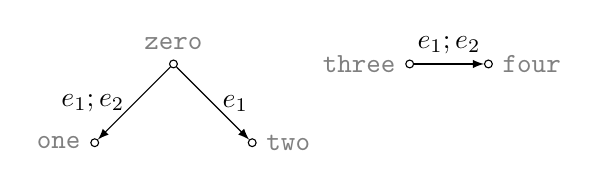
\begin{tikzpicture}
  \def\x{2.5}
  \tikzset{vertex/.style={draw,circle,inner sep=1pt}}
  \tikzset{transition/.style={->,>=latex}}
  \tikzset{every label/.style={gray}}
  \node[vertex] (zero) at (0,0) [label=above:\texttt{zero}] {};
  \node[vertex] (one) at (-1,-1) [label=left:\texttt{one}] {};
  \node[vertex] (two) at (1,-1) [label=right:\texttt{two}] {};

  \node[vertex] (three) at (3,0) [label=left:\texttt{three}] {};
  \node[vertex] (four) at (4,0) [label=right:\texttt{four}] {};

  \draw[transition] (zero)--node[left]{$ e_1;e_2$} (one);
  \draw[transition] (zero)--node[right]{$e_1$} (two);

  \draw[transition] (three)--node[above]{$e_1;e_2$} (four);
\end{tikzpicture}
\caption{Example of unmatched events.}
\label{fig:unmatched-example}
\end{figure}

\subsubsection{On labels and guards.} % <<<

A label is a list of pairs $(g,a)$ of guards and actions. A  {\em general guard} is a partial function of type:
\[
\set{GenGuard} = (\set{Pattern} \times \N \times \set{Pred}) \pmap (\set{Event}\times\set{Store}) \to \B
\]
An {\em instantiated guard} is a general guard provided with instances of a pattern  name $\pattern v$,  its position $i$ in the label, and a predicate $p$ needed to test this pattern:
\[
g_{\pattern{v},i,p} : \set{Event}\times\set{Store} \to \B
\]
Given an event and a store, an instantiated guard  evaluates whether the event satisfy the guard in the store. It is defined as:
\newcommand{\sem}[1]{[ \! | #1 | \! ]}
\[
g_{\pattern{v},i,p}(e, \sigma) = p(e[i],\sigma(\pattern v))
\] The guard is true if and only if the value of $\pattern{v}$ in the automaton store
and the value of $i$-th parameter of  event $e$ (obtained from the program store) satisfy $p$.
\begin{example}
%\rlp{Notation for not-guard should be unified ($\sim$ here ! earlier).}
Consider the label
 $ !\pattern {v} := \pattern {s}.gets(\pattern {k})$ to be matched with the statement
 {\tt t:=z.gets(h)}. Internally,  the label is compiled down to the
 following sequence of labels
\[
\pattern{call} \  \pattern{s}^0 .gets(\pattern {k}^1);  \ \pattern{ret} \ gets = ! \pattern {v}^0
\] where the upper-script stands for the position of a pattern in an
expression.
The statement, on the other hand, generates the trace of events $e_1 \cdot e_2$ where
\[
\begin{array}{l l}
 & e_1=(call \ gets, [0: \sem{z}, \ 1: \sem{h}])  \\
 \mbox{ and }  &  e_2= (ret \ gets, [0: \sem{t}]) 
\end{array}
\]
The instantiated guard for the label are:
 $g_{\pattern{s},0,=}$, $g_{\pattern{k},1,=}$, and  $g_{\pattern{v},0, \neq}$.
Notice that the predicates we want to use to compare patterns and events' values are: equality for the element $\pattern{s}$ and $\pattern{k}$,
but inequality for \pattern{v} (because of the negation $!$).
The instantiated guards, can now be evaluated with the events by taking their conjunction:
\[
 (tag(e_1)= \ call \ gets) \wedge g_{\pattern{s},0,=}(\sigma,e_1) \wedge g_{\pattern{k},1,=}(\sigma, e_1)
\] and
\[
 (tag(e_2)= ret \ gets) \wedge g_{\pattern{v},0,\neq}(\sigma,e_2).
\]
\end{example}

% >>>
% >>>
\section{From register automata to TOPL}
\rlp{Some definitions and theorems?}
\dd{Maybe explain the components of a register automaton} 
Given a register automaton~\cite{dblp:journals/tcs/kaminskif94} $A=\langle S, p, u, \rho, T,
F\rangle$, we will construct a TOPL property $P_A$ to simulate it. The
simulation is such that for each word $w$, $A$ accepts $w$ iff $P_A$
accepts $w' = \#^{|u|}w\#$. \dinocomment{what does it mean? what are the $\#$?} Thus, $w'$ is an encoding of $w$ that
caters for the differences of the two formalisms: A register automaton has an
initial state $u$ of length $|u|$. In order to set up the initial
state, the TOPL property needs to consume $|u|$ symbols, so we have to
put that many dummy symbols in front of the word. The dummy symbol at
the end is because $A$ may have many final states ($|F| > 1$) whereas a TOPL
property only has one, so we need to make an extra transition from all
the erroneous states to the actual error state.

%\begin{definition}
%Let $A=\langle S, p, u, \rho, T, F\rangle$ be an FSA
%\end{definition}
\newcommand{\Vertex}{\mathit{Vertex}}
\newcommand{\Arc}{\mathit{Arc}}
To construct the TOPL property we have to define the set $\Vertex$
of vertices and the set $\Arc$ of labelled transitions. We do that as follows:
\[
\Vertex = S \cup \{start, error\}
\]
that is we have the same set of vertices as $A$ plus two new
ones. $start$ is going to be the initial vertex. It will have a
transition to the start vertex $p$ of $A$ that sets up the
initial state. Thus, if $u = w_1\ldots w_n$, then Arc includes
\[
A_{start} = start \to p: (*,R_1=w_1);\ldots;(*,R_n=w_n)
\]
a transition of depth $n = |u|$ that assigns the letters of $u$
to $n$ automaton variables. The guard $*$ simply ignores the
event\footnote{One could also chose a guard that forces the event
to be \#.}. This transition consumes the first $n$ extra
symbols. $\Arc$ further includes
%\[
%\forall (s, i, s') \in T.\ s\to s': r_i=e, skip
%\]
\[
A_{seen} = \bigcup_{(s, i, s') \in T} s\to s': r_i=e, skip
\]
coresponding to the case where $e$ has been seen before, and
%\[
%\forall (s, i, s') \in T.\ \rho(s)=i.\ s\to s': unknown(e), R_i=e
%\]
\[
A_{unseen} = \bigcup_{(s, i, s') \in T,\ \rho(s)=i} s\to s': unknown(e), R_i=e
\]
where $unknown(e) = r_1 \neq e \land \ldots \land r_n \neq e$,
coresponding to the case where $e$ has not been seen (or has been
forgotten). In this case, the relevant register is
updated. Finally $\Arc$ includes
%\[
%\forall s\in F.\ s\to error: *, skip
%\]
\[
A_{error} = \bigcup_{s\in F} s\to error: *, skip
\]
to send the vertices in $F$ to the error state. This transition
consumes the final extra symbol.

Formally, we can define
\[
\mathrm{Arc} = A_{start} \cup A_{seen} \cup A_{unseen} \cup A_{error}.
\]

% >>>
\section{Implementation} \label{sec:implementation} % <<<

Our tool\footnote{\url{http://rgrig.github.com/topl}} checks whether a Java program violates a TOPL property.
The tool consists of two parts: a compiler and a checker.
The TOPL compiler ({\tt toplc}) instruments Java bytecode;
The TOPL checker (class {\tt topl.Checker}) monitors the execution and reports violations.
\autoref{architecture} depicts how the compiler and the checker fit together, thus summarizing our runtime checking technique.

\begin{figure*}[t]
\begin{center}
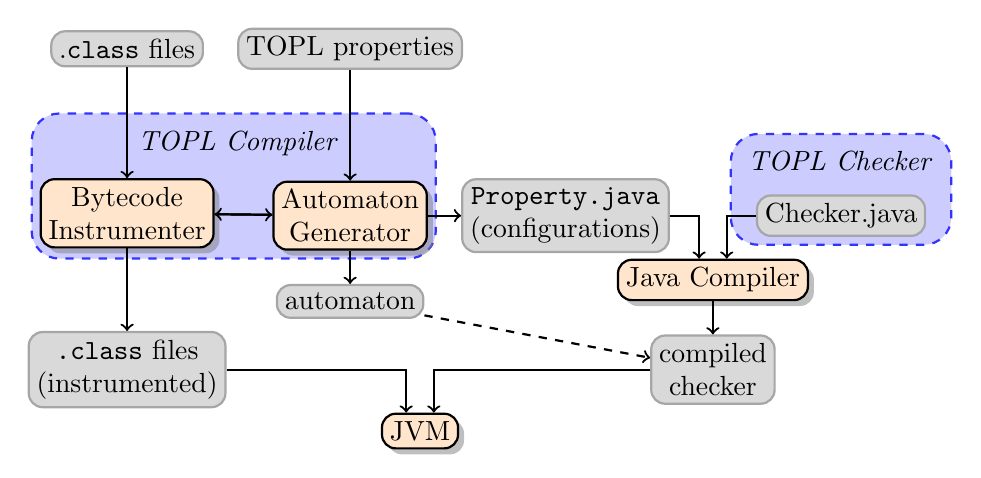
\begin{tikzpicture}[node distance=12pt, auto]
\tikzstyle{system}=[rectangle,
                                draw=blue!80,
                                fill=blue!20,
                                inner sep=0.1cm,
                                rounded corners=10pt,
                                style=dashed,thick]
\tikzstyle{program}=[rectangle,
                                  draw=black,
                                  fill=orange!20,
                                  inner sep=0.1cm,
                                  rounded corners=5pt,
                                  style=thick,
                                  drop shadow]
\tikzstyle{data}=[rectangle,
                            draw=gray!70,
                            fill=gray!30,
                            inner sep=0.1cm,
                            rounded corners=5pt,
                            style=thick]
\node[data] (classes) {{.\tt class} files};
\node[data, right=of classes] (properties) {TOPL properties};

\node[below=of classes] (classesd) {};
\node[below=of properties] (propertiesd) {};

\node[program, below=40pt of classes, align=center] (instrumenter)
  {Bytecode\\Instrumenter};
\node[program, below=40pt of properties, align=center] (genautomaton)
  {Automaton\\Generator};

\node[data, right=of genautomaton, align=center] (javaproperties)
  {{\tt Property.java}\\(configurations)};
\node[data, below=of genautomaton] (automaton) {automaton};
\node[right=of javaproperties] (javadummy) {};
\node[data, right=of javadummy] (checker) {Checker.java};
\node[program, below=of javadummy] (javac) {Java Compiler};

\node[data, below=of javac, align=center] (classproperties)
  {compiled\\checker};
\node[data, align=center] at (instrumenter |- classproperties)
  (instrclasses) {{\tt .class} files\\(instrumented)};
\node at ($(instrclasses)!.5!(classproperties)$) (classdummy) {};
\node[program, below=of classdummy] (jvm) {JVM};

\node[above=5pt] at ($(instrumenter.north)!.5!(genautomaton.north)$) (topllabel) {\emph{TOPL Compiler}};
\node[above=5pt of checker] (checkerlabel) {\emph{TOPL Checker}};
\begin{pgfonlayer}{background}
  \node[system, fit = (topllabel) (instrumenter) (genautomaton)] (TOPLC) {};
  \node[system, fit = (checker) (checkerlabel)] (CHECKER) {};
\end{pgfonlayer}

\path[thick, ->]
(classes) edge (instrumenter)

(genautomaton) edge (instrumenter)
(instrumenter) edge (genautomaton)

(properties) edge (genautomaton)
(genautomaton)  edge (javaproperties)
(javac) edge (classproperties)

(genautomaton) edge (automaton)

(instrumenter) edge (instrclasses);

\draw[thick, ->]
(instrclasses) -| ($(jvm.north)-(5pt,0)$);
\draw[thick, ->]
(classproperties) -| ($(jvm.north)+(5pt,0)$);
\draw[thick, ->]
(javaproperties)  -| ($(javac.north)-(5pt,0)$);
\draw[thick, ->]
(checker)  -| ($(javac.north)+(5pt,0)$);

\draw[thick, ->, dashed]
(automaton) -- (classproperties);
(\end{tikzpicture}

\caption{Architecture of the TOPL tool}
\label{architecture}
\end{center}
\end{figure*}

The compiler takes as input a Java project and a set of TOPL properties.
The Java project is defined to be all files in a given directory, recursively descending into jar files, zip files, and subdirectories.
The compiler produces (1)~a copy of the Java project with the class files instrumented, and (2)~a TOPL automaton.
The bytecode instrumentation and the construction of the TOPL automaton are intertwined.
On one hand, only the Java methods relevant to the given TOPL properties are instrumented.
On the other hand, the construction of the TOPL automaton relies on the inheritance tree of the Java project.
For example, suppose that a TOPL property mentions the method {\tt next} from the interface {\tt Iterator}.
Then, on one hand, all the methods that implement {\tt Iterator.next} are instrumented and, on the other hand, the corresponding guard in the automaton will match all these methods.

The compiler also performs two secondary tasks, for convenience.
First, it inserts a copy of the checker in the instrumented version of the Java project.
Second, it generates a Java file that activates and configures the checker.
It is this file that must be recompiled if one wishes to change the parameters of the checker, such as the maximum number of active states to track.
Because of these convenience features, all the user needs to do next is run the instrumented version of the Java project.

The checker logs property violations to {\tt System.err}.
The configuration parameters of the checker include:
\begin{itemize}
\item \emph{History length}---how many events to remember.
  A high value reports more events that led to \error.
  A low value reduces the space and time overhead.
\item \emph{Maximum number of active states}.
  A high value increases the chances of detecting violations.
  A low values reduces space and time overhead.
\item \emph{Collect call stacks}.
  A {\tt true} value includes call stacks in violation reports.
  A {\tt false} value reduces the space and time overhead.
\end{itemize}

\subsection{The TOPL Compiler} \label{sec:toplc} % <<<

The compiler has six phases, which are described below.

\paragraph{Parsing and Desugaring.}
TOPL properties are read first, before the Java project.
The parser desugars the TOPL properties into a simpler, intermediate form where
\begin{itemize}
\item Method-name patterns are prefixed according to the {\tt prefix} directive.
\item Lowercase patterns and constant patterns are turned into guards.
\item Uppercase patterns are turned into actions.
\item Transitions of length 2 or of length 1 are built according to whether the guards and the actions refer to both call-time and return-time or not. (In particular, there are no transitions of length~$0$.)
\end{itemize}
The parser builds an AST that closely follows the language for which we gave formal operational semantics.

\paragraph{Static Checks.}
Next, the compiler checks that the property is well-formed:
\begin{itemize}
\item two parallel writes to automaton variables have distinct destinations;
\item reads from automaton variables must be preceded by writes.
\end{itemize}

The compiler warns if some vertices are unused.
Properties with unused vertices are still well-formed.
We plan to also statically check whether the automaton can never fail.

\paragraph{Generate Event Identifiers.}

In this phase, each observable method is assigned two identifiers, one for the call event and one for the return event.
A method is \emph{observable} when its full name or the full name of a method it overrides matches the {\tt observe} directive.
The bytecode is read to collect all method names and to build the inheritance tree.

\paragraph{Construct the Automaton.}

In this phase, all properties are merged into one automaton.
From now on vertices are integers, rather than strings.
All vertices that had the name \start are now in the set of start vertices;
all vertices that had the name \error now have an error message attached.
Each TOPL property has its own {\tt observe} directive.
This information must be encoded in the automaton:
Each vertex is given a set of event identifiers.

The guards of the automaton are of two kinds.
Those that test program values are essentially left unchanged in this phase.
Those that check the event type, the method name, and the method arity are all transformed into one guard that is represented by a set of event identifiers.
The evaluation of the guard at runtime is a set containment test.

The automaton is dumped into the file {\tt Property.text}.
The TOPL compiler does not interpret Java expressions.
If a guard compares a program value with a literal, then the literal is saved in an array in {\tt Property.java}, and {\tt Property.text} points to it.

\paragraph{Generate Checker Configurations.}

In this phase, which is intertwined with the previous one, the compiler generates a file {\tt Property.java}.
This file serves three purposes:
\begin{itemize}
\item
It contains an array with all the constants used in the TOPL property.
For example, if a guard requires that a certain argument equals the expression~$21/7$, then $21/7$ is stored in this array.
\item
It activates the checker.
The checker is inactive by default so that the Java standard library may be instrumented.
The JVM uses certain parts of the standard library during its own startup.
If those parts happen to be instrumented then they call into the checker.
If the checker is inactive it immediately returns and the execution continues.
If the checker would be active then it will call back into the standard library and the JVM will crash.
\item
For convenience, it contains code that configures the checker.
To change the parameters of the checker the user changes this code and recompiles {\tt Property.java}.
\end{itemize}

\paragraph{Instrumentation.}

In this phase, the bytecode of observable methods is instrumented.
The first and last actions performed by the instrumented version are calls to the method {\tt check} of the checker.
This method takes an event as an argument.
Each event carries an identifier and an array of {\tt Object}.
The array holds either the arguments, or the return value.

To instrument Java bytecode we use a fork of the library Barista~\cite{barista}.
The high-level bytecode representation of the original library is rather low-level.
For example, it still represents jumps as byte counts.
We changed Barista's high-level representation to make it easy to use for instrumentation.
Hence, we had to rewrite the code that transformed between the low-level and the high-level representation.
These changes amount to more than half our implementation effort.
(For example, adding the number of lines changed by each commit gives $48\rm\,K$.)

% >>>
\subsection{The TOPL Checker} % <<<

The checker logs the property violations that it detects.
Its components are:
\begin{itemize}
\item the data structures used to represent the automaton, and a parser that instantiates them while processing {\tt Property.text};
\item the data structures used to represent the current state of the checker;
\item the code that handles one incoming event;
\item the code that garbage collects old states; and
\item the code that chooses which of the active states to forget.
\end{itemize}

\paragraph{States.}
The checker maintains a set of active states.
A state consists of vertex, a store, and a queue of events yet to be processed.
The vertex is simply an integer.
The store maps automaton variables ({\tt in}) to values ({\tt Object}).
A maximum size of~$2$ for the queue of events suffices because transitions have depth $1$~or~$2$.
(If all transitions would have the same depth, then one global queue of events would suffice.
Since the transition depth is bounded the checker could still use a couple of global queues, but we chose for now an implementation that is easy to generalize.)

States are created produced by applying an action to another state (called the parent).
For error reporting, each state keeps track of its parent.
An active state with $\ge2$~outgoing transitions produces $\ge2$~active states for the next time step.
The new active states and their parent are likely to have similar stores.
The implementation takes advantage of this fact by using persistent (functional) sets for bindings to represent stores; more precisely, we use treaps~\cite{DBLP:conf/focs/AragonS89}.

\paragraph{Step.}

The procedure from \autoref{fig:checker.step} builds the set~$A$ of states that are active after processing one event.
It corresponds to the operational semantics (\autoref{sec:semantics}), but is written in an imperative style.
For each transition outgoing from a vertex, lines~\hbox{11--17} try to apply rule (Step) from \autoref{sec:semantics}.
Line~17 is reached if the rule (Step) does not apply, and execution continues with the next outgoing transition.
Line~18 is reached if the rule (Step) does apply.
Its effect is recorded by adding a new state to set~$A$
If rule (Step) did not apply for any outgoing transition, then rule (Silent) is applied by lines~22--23.

\begin{figure*}[t]
\begin{center}
\begin{alg}
\^  $\proc{Step}(e)$
\=  $A := \emptyset$
\=  for each active state $s$
\+    if $\mathit{vertex}(s)$ does not observe $\mathit{id}(e)$
\+      insert $s$ into $A$
\=      continue from $3$
\-    push $e$ to the queue $\mathit{events}(s)$
\=    if $\mathit{events}(s)$ is shorter than the longest transition from $\mathit{vertex}(s)$
\+      continue from $3$
\1    $\mathit{skip}:=\mathsf{true}$
\=    for each transition $t$ outgoing from $\mathit{vertex}(s)$
\+      $\sigma := \mathit{store}(s)$,\quad $E := \mathit{events}(s)$
\=      for each step $\tau$ of $t$
\+        pop $\varepsilon$ from the queue $E$
\+        if $\proc{Guard}(\tau, \varepsilon, \sigma)$
\+          $\sigma := \proc{Action}(\tau, \varepsilon, \sigma)$
\-        else
\+          continue from 11
\2      $\mathit{skip}:=\mathsf{false}$
\=      insert state $(\mathit{target}(t), \sigma, E)$ into $A$
\=      if $\mathit{target}(t)$ is an error vertex, report the error
\=      if \textit{skip}
\+        $s' := s$
\=        insert state $s'$ with one event popped into $A$
\end{alg}
\bigskip
\caption{
  Executing one step.
  The code builds the set~$A$ of states that are active after processing one event.
}
\label{fig:checker.step}
\end{center}
\end{figure*}

\paragraph{Garbage Collection.}

States point to their parent when they are created.
But, if they continue to do so forever, then the memory footprint of the states would be proportional to the number of events received by the checker.
The space overhead would be too big for long running programs.
Usually, most of the states are not needed.
The typical property has a $*$-loop on the \start vertex.
An error trace going all the way back to the beginning would mention that this loop is taken many times before something interesting happens.
In general it is very unlikely that the user needs a trace with more than about $10$~states.
The history length~$h$ is one of the parameters configurable from {\tt Property.java}.

We should allow the Java~VM to garbage collect states that are not reachable in $h$~steps from some active state.
After each {\sc Step} we could do a BFS traversal with $h$~steps and set to {\tt null} the parent pointer of fringe states.
However, if there are $n$~active states, the traversal would take $O(nh)$~time.
The procedure {\sc Step} takes $O(nd)$~time, where $d$ is the maximum out-degree of the property.
So, the checker would become much slower if $h>d$, which usually is the case.

One solution could be to perform the BFS once in every $h/d$~steps.
The solution we implemented tries to better address the average case.
We remember the number~$m$ of states seen by a BFS, and perform the next BFS after $\sim m$~new states were created.

\paragraph{Approximation.}

\autoref{fig:completeness} illustrates why the checker needs unbounded memory if it must not miss bugs exhibited by an execution.
The problem is essentially that the set of active states of a nondeterministic automaton is unbounded.
Of course, an arbitrary amount of space overhead is unacceptable.

\begin{figure}[t]
\begin{center}
\begin{Verbatim}[commandchars=\\\{\}]
\PY{k+kn}{import} \PY{n+nn}{java.util.*}\PY{o}{;}
\PY{k+kd}{public} \PY{k+kd}{class} \PY{n+nc}{Completeness} \PY{o}{\PYZob{}}
   \PY{n}{Collection} \PY{n}{c}\PY{o}{;}
   \PY{n}{Random} \PY{n}{r}\PY{o}{=}\PY{k}{new} \PY{n}{Random}\PY{o}{(}\PY{o}{)}\PY{o}{;}
   \PY{k+kd}{public} \PY{k+kt}{void} \PY{n+nf}{NeedsUnboundMemory}\PY{o}{(}\PY{k+kt}{int} \PY{n}{n}\PY{o}{)} \PY{o}{\PYZob{}}
      \PY{n}{Iterator}\PY{o}{[}\PY{o}{]} \PY{n}{a} \PY{o}{=} \PY{k}{new} \PY{n}{Iterator}\PY{o}{[}\PY{n}{n}\PY{o}{]}\PY{o}{;}
      \PY{k}{for} \PY{o}{(}\PY{k+kt}{int} \PY{n}{i}\PY{o}{=}\PY{l+m+mi}{0}\PY{o}{;} \PY{n}{i}\PY{o}{<}\PY{n}{n}\PY{o}{;} \PY{n}{i}\PY{o}{+}\PY{o}{+}\PY{o}{)} \PY{o}{\PYZob{}}
          \PY{n}{a}\PY{o}{[}\PY{n}{i}\PY{o}{]}\PY{o}{=}\PY{n}{c}\PY{o}{.}\PY{n+na}{iterator}\PY{o}{(}\PY{o}{)}\PY{o}{;}
          \PY{k}{if} \PY{o}{(}\PY{n}{r}\PY{o}{.}\PY{n+na}{nextBoolean}\PY{o}{(}\PY{o}{)}\PY{o}{)} 
	    \PY{k}{while} \PY{o}{(}\PY{n}{a}\PY{o}{[}\PY{n}{i}\PY{o}{]}\PY{o}{.}\PY{n+na}{hasNext}\PY{o}{(}\PY{o}{)}\PY{o}{)} \PY{n}{a}\PY{o}{[}\PY{n}{i}\PY{o}{]}\PY{o}{.}\PY{n+na}{next}\PY{o}{(}\PY{o}{)}\PY{o}{;}	
      \PY{o}{\PYZcb{}}\PY{o}{;}
      \PY{n}{a}\PY{o}{[}\PY{n}{r}\PY{o}{.}\PY{n+na}{nextInt}\PY{o}{(}\PY{n}{n}\PY{o}{)}\PY{o}{]}\PY{o}{.}\PY{n+na}{next}\PY{o}{(}\PY{o}{)}\PY{o}{;}
  \PY{o}{\PYZcb{}}\PY{o}{;}
\PY{o}{\PYZcb{}}
\end{Verbatim}

\caption{Counterexample to runtime completeness.}
\label{fig:completeness}
\end{center}
\end{figure}

Like in the case of trace lengths, we impose a limit that is fixed but configurable by the user.
In this case, however, we must also pick which active states to forget.
We implemented three strategies: random, newest, and oldest.
The words newest\slash oldest refer to a time that is attached to states, and is one more than the time of the parent state.
The time of a state is the number of times the (Step) transition of the operational semantics was taken in order to produce the state.

%\dinocomment{discuss about: conservative and transparent properties of an inliner}
%\dinocomment{talk about our strategy}

% >>>
% >>>
\section{Related Work}\label{sec:related} %<<<

TOPL takes inspiration from several existing  languages for type-state~\cite{strom1986,dblp:conf/oopsla/bierhoffa07,dblp:conf/oopsla/naeeml08,disney2011,ball2002}, but  it allows articulating  relationships and interactions among several objects.
Existing techniques for type-state aim at decomposing properties involving several objects into specifications reflecting the point of view of {\em one} single object.
TOPL, in contrast,  intentionally avoids such decomposition.
Parkinson~\cite{parkinson-iwaco2007} argues that invariants involving several objects are often better than one-object invariants.
Similarly, we believe that temporal properties that naturally involve a plurality of objects are easier to express and reason about if they are \emph{not} decomposed.
One language in the literature sharing this point of view is tracematches~\cite{dblp:conf/oopsla/allanachklmsst05}.
The ability of TOPL automata to store,  update, and compare values of their (infinite alphabet) registers combined with nondeterminism makes TOPL strictly more expressive than tracematches.

TOPL properties are based on register automata~\cite{dblp:journals/tocl/demril09}.
Compared to this formalism, a major difference is that in TOPL automata, transitions can be taken based upon sequences of events of different size.
For runtime checking this requires a sort of backtracking to fire different transitions for different  sequences of events.
On a static setting this phenomenon is normally encoded using non-determinism combined with prophecy variables~\cite{dblp:journals/tcs/abadil91}.

Our work 
extends the fundamental concept 
of typestate~\cite{strom1986} originally developed for imperative programs
by integrating notions typical of object-oriented programs.
 We are certainly not the first in doing this: there are several extensions of typestate to object-oriented programming in the literature.
A modular static verification method for typestate protocols is introduced in~\cite{dblp:conf/oopsla/bierhoffa07}.
The specification method is based on linear logic and relations among objects in the protocol are monitored by a tailored system of permissions.
The method is highly modular and presumably efficient.
The specification of the interactions among objects by means of permissions adds an extra level of machinery which increases the gap between the intuitive protocol description and its formalization.
Similarly~\cite{deline2004,dblp:conf/sigsoft/BierhoffA05} provide a mean to specify typestate properties that belong to a single object.
The specified properties are reminiscent of contracts or pre/post-conditions for methods and can deal with inheritance.
In~\cite{dblp:conf/issta/FinkYDRG06} the authors present sound verification techniques for typestate properties of Java  programs.
Their approach is divided in several stages with different verifiers varying for cost and precision.
In the early stages efficient but imprecise analyses are employed whereas more expensive and precise techniques are then progressively employed in later stages.
Every stage focuses on verifying only the parts of the code that previous stages failed to verify.
It is likely that  TOPL could be fruitfully combined with their analysis technique.

QVM~\cite{arnold:2008} is a runtime monitoring system tracking a subset of objects, chosen by
sampling. To ensure that the timing overhead of the monitoring is below a given target, the sampling rate is 
automatically adapted on the fly. For TOPL the control of the overhead is done manually by  the programmer who can tune the quantity of info to be tracked.
To improve performance,  the implementation of the QVM monitor is in the virtual machine,which, as a consequence makes it less portable for
different virtual machines. 
%\dd{how do we defend ourselves for the fact that we cannot predict
%  overhead?}\rlp{by experiments?}
An automata-based formalism for specifying properties of software interfaces was introduced in~\cite{dblp:conf/sigsoft/AlfaroH01} .
This language aims at capturing assumptions about the order in which the methods of a component are called and the order in which the component calls external methods.
In contrast to TOPL, this formalism is mainly used to check the compatibility of the interfaces of two components and it is designed to be applied at  model level rather than code level.
A specification language for interface checking aimed at C programs (called SLIC) is introduced in~\cite{ball2002}.
Differences between SLIC and TOPL include: the use (in SLIC) of non-determinism to encode universal quantification of dynamically allocated data, and the  ability to have complex code in the automaton transitions.
TOPL specifications naturally express universally quantified properties over data structures and for computability reasons,  we have chosen to limit the  actions performed during automaton transitions.
Simple SLIC specifications are verified by  the SLAM verifier~\cite{dblp:conf/cav/ballr01}.
While SLAM specialises on device drivers and checks client conformance rather than full protocols,
very general specifications of object-oriented program behaviour can be given in JML~\cite{jml} and Spec$\sharp$~\cite{DBLP:journals/jot/BarnettDFLS04}. However the latter two languages focus on class specifications and do not have temporal features.

In~\cite{disney2011} contracts are used to express legal traces of programs in a functional language with references.
The contracts specify traces as regular expressions over calls and returns, and hence, they resemble our automata, in a quite different setting.
Here, the specifications are function-centered, though, and again, capturing inter-object relations seems somewhat tricky.

ConSpec~\cite{DBLP:journals/entcs/AktugN08} is a language used to describe security policies.
Because ConSpec automatons are deterministic and have only a countable number of states, they cannot in principle express the property \texttt{InvalidateOtherIterators} (\autoref{sec:examples.steps}).


%\rg{I think the paper~\cite{dblp:journals/tocl/demril09} adds an operator to LTL to make it more expressive than register automata.
%We should discuss here, but I moved the citation out of the introduction.}
%\dinocomment{Add more on dynamic checks and byte code instrumentation}
%\dd{cite grigore rosu's work}
% >>>
\section{Conclusions and Future Work}\label{sec:conclusions} %<<<

\paragraph{Conclusions.}
We introduced TOPL---a language for expressing temporal safety properties for object-oriented programs via an extension of register automata.
TOPL can express constraints involving the relation of many objects at the same time.
Furthermore, we introduced a technique for checking at runtime the violation of the properties on Java program.
We have applied our technique to a variety of programs including large open source Java projects.
%
\paragraph{Future work.}
In the future, we intend to combine TOPL with  separation logic~\cite{reynolds2002} in order to deal with the heavy use of the heap and aliasing in object-oriented software.
Moreover, we aim at developing static analysis techniques for TOPL properties using the jStar framework~\cite{DBLP:conf/oopsla/DistefanoP08}.
This will require investigating suitable abstraction for obtaining meaningful and precise over-approximations of the state space of the programs.
Finally, we intend to develop a tailored bi-abduction inference technology~\cite{dblp:conf/popl/CalcagnoDOY09} which would help with scalability of the analysis.
%\rlp{What about abstraction even for dynamic analysis?}
%>>>
\bibliographystyle{plain} % and appendix <<<
\bibliography{safety}

\appendix
\section{TOPL Syntax}
\label{app:syntax}
\begin{tabular}{l}
\grammar{
  Property& \b{property} Identifier Item\* \cr
  Item& Prefix \| Observe \| Transition \cr
  Prefix& \b{prefix} \b< StringPattern \b> \cr
  Observe& \b{observe} \b< StringPattern \b> \cr
  Transition& Arc \b: Label \(\b, Label\)\* \cr
  StringPattern& \(Letter \| \b. \| \b* \| \b{\{} \| \b{\}} \| \b, \)\+ \cr
  Arc& Vertex \b{->} Vertex \cr
  Label& Tag\? MethodPattern \cr
  Vertex& Identifier \cr
  Tag& \b{call} \| \b{return} \cr
  MethodPattern& ResultPattern\? NamePattern ArgumentsPattern \cr
  ResultPattern& ValuePattern \b{:=} \cr
  NamePattern& StringPattern \cr
  ArgumentsPattern& \b( \(ValuePattern \(\b, ValuePattern\)\*\)\? \b) \cr
  ArgumentsPattern& \b[ IntegerPattern \b] \cr
  ValuePattern& \b* \| \b< Literal \b> \| UppercaseId \| LowercaseId \cr
  IntegerPattern& \b* \| IntegerLiteral \cr
}
\end{tabular}


\begin{figure*}[h]\label{fig:tomcat-prop}
\begin{Verbatim}
property InterleavedResponse2
  // vertex names: w = got writer; W = used writer; similarly for s, S
  message "Incompatible methods for putting data into a response were used."
  observe <javax.servlet.ServletOutputStream.*>
  observe <java.io.PrintWriter.*>
  observe <javax.servlet.ServletResponse.{getOutputStream,getWriter}>
  prefix <javax.servlet.ServletResponse>
  start -> start: *
  start -> w: W := R.getWriter()
  start -> s: S := R.getOutputStream()
  w -> sw: S := r.getOutputStream()
  s -> sw: W := r.getWriter()
  w -> W: w.*
  sw -> sW: w.*
  s -> S: s.*
  sw -> Sw: s.*
  W -> sW: S := r.getOutputStream()
  S -> Sw: W := r.getWriter()
  sW -> error: s.*
  Sw -> error: w.*
\end{Verbatim}
\caption{Example Tomcat Propery}
\end{figure*}

% >>>
\end{document}
%% vim:spell errorformat=%f\:%l-%m,%f\:%l\:%m,%f\:%m
%% vim:fmr=<<<,>>>:
